\documentclass{IOS-Book-Article}

\usepackage{cite}
\usepackage{mathptmx}

\usepackage[pdftex]{graphicx}
% declare the path(s) where your graphic files are
% \graphicspath{{../pdf/}{../jpeg/}}
% and their extensions so you won't have to specify these with
% every instance of \includegraphics
\DeclareGraphicsExtensions{.pdf,.jpeg,.png}

\usepackage{url}

\def\hb{\hbox to 10.7 cm{}}

\newcommand{\psykal}{{PS}y{KA}l\ }

%%%%%%%%%%%%%%%%%%%%%%%%%%%%%%%%%%%%%%%%%%%%%%%%%%%%%%%%%%%%%%%%%%
\begin{document}

\pagestyle{headings}
\def\thepage{}

\begin{frontmatter}              % The preamble begins here.
%
% can use linebreaks \\ within to get better formatting as desired
\title{Towards Compiler-Agnostic Performance in Finite-Difference Codes}

\author[A]{\fnms{A. R.} \snm{Porter}%
\thanks{Corresponding Author: Andrew Porter, STFC Daresbury Laboratory, Warrington, WA4 4AD, UK; E-mail:
andrew.porter@stfc.ac.uk.}},
\author[A]{\fnms{R. W.} \snm{Ford}},
\author[A]{\fnms{M.} \snm{Ashworth}},
\author[B]{\fnms{G. D.} \snm{Riley}}
and
\author[C]{\fnms{M.} \snm{Modani}}
\runningauthor{A.~R.~Porter et al.}
\address[A]{STFC Daresbury Laboratory, Warrington, WA4 4AD, UK}
\address[B]{The University of Manchester, UK}
\address[C]{STFC Hartree Centre}

\begin{abstract}
In this paper we evaluate the performance implications of applying a
technique which we call \psykal to finite difference Ocean models. 
%
In \psykal, the code related to the underlying science is formally
separated from code related to parallelisation and single core
optimisations. This separation of concerns allows scientists to code
their science independently of the underlying hardware architecture
(thereby keeping a single code base) and for optimisation specialists
to be able to tailor the code for a particular machine independently
of the science code.
%
A finite difference shallow water benchmark optimised for cache based
architectures is taken as the starting point. A vanilla \psykal version
is written and the performance of the two compared. The optimisations
that were applied to the original benchmark (loop fusion {\it etc.}) are then
applied to the \psykal version as a set of code modifications to the
optimisation layer. Performance results are presented for the Cray,
Intel and GNU compilers on Intel Ivybridge and Haswell processors and
for the IBM compiler on Power8.
%
Results show that the combined set of code modifications obtain
performance that is within a few percent of the original code for all
compiler and architecture combinations on all tested problem
sizes. The only exception to this (other than where we see significant
speed-ups) is the Gnu compiler on Haswell for one problem size. Our
tests indicate that this may be due to immature support for that
architecture in the Gnu compiler -- no such problem is seen on the Ivy
Bridge system.
%%
Therefore, the \psykal approach can be used with negligable
performance loss and sometimes small performance gains compared to the
original optimised code, there is no single best hand optimised
implementation of the code for all the compilers tested, and the
flexibility in applying code modifications to the optimisation layer
in the PSyKAl version allows for a significant performance improvement
on the IBM Power8 compared with the original code.

\end{abstract}

\begin{keyword}
Performance, Code-generation, Finite-difference
\end{keyword}

\end{frontmatter}

%%%%%%%%%%%%%%%%%%%%%%%%%%%%%%%%%%%%%%%%%%%%%%%%%%%%%%%%%%%%%%%%%%%%
% Introduction is not to be numbered so use \section*{}
\section*{Introduction}
The challenge presented to the developers of
scientific software by the drive towards Exascale computing is
considerable. With power consumption becoming the overriding design
constraint, CPU clock speeds are falling and the complex,
multi-purpose compute core is being replaced by multiple, simpler
cores. This philosophy can be seen at work in the rise of so-called
accelerator based machines in the Top 500 List~\cite{top500} of
supercomputers: five of the top-ten machines in the November 2014 list
make use of Intel Xeon Phi's or NVIDIA GPUs. Four of the remaining
five machines in the top ten are IBM BlueGene/Qs, the CPU of which has
hardware support for running 64 threads.

Achieving good performance on large numbers of light-weight cores
requires exploiting as much parallelism in an application as possible
and this results in increased complexity in the programming models
that must be used. This in turn increases the burden of code
maintenance and code development, in part because two specialisms are
required: that of the scientific domain which a code is modelling
({\it e.g.} oceanography) and that of computational science. The
situation is currently complicated still further by the existence of
competing hardware technology; if one was to begin writing a major
scientific application today it is unclear whether one would target
GPU, Xeon Phi, traditional CPU, FPGA or something else entirely. This
is a problem because, generally speaking, these different technologies
require different programming approaches.

\subsection*{The \psykal Approach}

The \psykal approach attempts to address the problems described in the
previous section. It separates code into three layers; the Algorithm
layer, the PSy layer and the Kernel layer. The approach has been
developed in the GungHo project~\cite{GungHo}, which is creating a new
Dynamical core for the Met Office, and its design has been influenced
by earlier work on OP2~\cite{OP2,PYOP2}.

While this approach is general, we are currently applying it to
Atmosphere and Ocean models written in Fortran where domain
decomposition is typically performed in the latitude-longitude
direction, leaving columns of elements on each domain-decomposed
partition.

The top layer, in terms of calling hierarchy, is the Algorithm
layer. This layer specifies the algorithm that the scientist would like
to perform (in terms of calls to kernel and infrastructure routines)
and logically operates on full fields. We say logically here as the
fields may be domain decomposed, however the algorithm layer is not
aware of this. It is the scientist's responsibility to write this
algorithm layer.

The bottom layer, in terms of calling hierarchy, is the Kernel
layer. The Kernel layer implements the science that the Algorithm
layer calls, as a set of subroutines. These kernels operate on fields
that are local to the process doing the computation. (Depending on the
type of kernel, these may be a set of elements, a single column of
elements, or a set of columns.). Again the scientist is responsible
for writing this layer and there is no parallelism specified here,
but, depending on the complexity of the Kernels, there may be input
from an HPC expert and/or some coding rules to help ensure the kernels
compile into efficient code.

The PSy layer sits in-between the Algorithm and Kernel layers and its
functional role is to link the algorithm calls to the associated
kernel subroutines. As the Algorithm layer works on logically global
fields and Kernel layer works on local fields, the PSy layer is
responsible for iterating over columns. It is also responsible for
including any distributed-memory operations resulting from the
decomposition of the simulation domain, such as halo swaps and
reductions.

As the PSy layer iterates over columns, the single core performance
can be optimised by applying transformations such as loop fusion and
loop blocking. Additionally, the potential parallelism within this
iteration space can also be optimised and parallelised. The PSy layer
can therefore be tailored for a particular hardware (such as
multi-core, many-core, GPGPUs, or some combination thereof) and
software (such as compiler, operating system, MPI implementation)
configuration with no change to the algorithm or kernel layer
code. This approach therefore offers the potential for portable
performance.

Clearly the separation of code into distinct layers may have an effect
on performance. This overhead, how to get back to the performance
of a hand-optimised code, and potentially improve on it, will be
discussed in the remainder of this paper.

\subsection*{The `Shallow' Program}

For this work we use a benchmark called Shallow which solves the
shallow-water equations on a bi-periodic plane following the
finite-difference scheme introduced by Sadourny~\cite{sadourny75}.
This software was originally written in 1984 by Paul Swarztrauber of
the National Center for Atmospheric Research, US.  However, in common
with many scientific codes, it has subsequently undergone some sort of
evolutionary development with subsequent people making various changes
and optimising it for previous generations of hardware.  There is no
complete record of the people involved and the precise hardware they
were targetting. In describing our work, we term the version of the
Shallow program obtained at the beginning of this project the
`original' version.

Shallow is a very good test case for our purposes since the original
version is short (some 600 lines) and contained within a single source
file. This makes it relatively straightforward for a compiler to
optimise. Its performance is thus quite a demanding target for our
modified versions of the code to reproduce.

Since any real oceanographic computational model must output results,
we ensure that any \psykal version of Shallow retains the Input/Output
capability of the original (it reads the problem specification from a
namelist and outputs the solution fields every $n$ timesteps). This
aids in limiting the optimisations that can be performed on the
\psykal version to those that should also be applicable to full
oceanographic models. Note that although we retain the I/O
functionality, all of the results presented in this work carefully
exclude the effects of I/O since it is compute performance that
interests us here.

In order to maximise the flexibility (and thus potential for
optimisation) of the \psykal version of Shallow, we made the kernels
as fine-grained as possible. In this case, this resulted in eight
distinct kernels, each of which operated on a single field at a single
point (since we have chosen to use point-wise kernels). With a little
bit of tidying/re-structuring, we found it was possible to express the
contents of the main time-stepping loop as a single invoke (a call to
the PSy layer) and a call to the I/O system
(Figure~\ref{FIG_psykal_shallow_structure}). The single PSy-layer
routine then consists of applying each of the kernels to all of the
points on the model mesh requiring an update. In its basic,
unoptimised (`vanilla') form, this PSy-layer routine then contains a
doubly-nested loop around each kernel call, as indicated by the
pseudo-code in Figure~\ref{FIG_psykal_shallow_structure}.

\begin{figure}
\centering
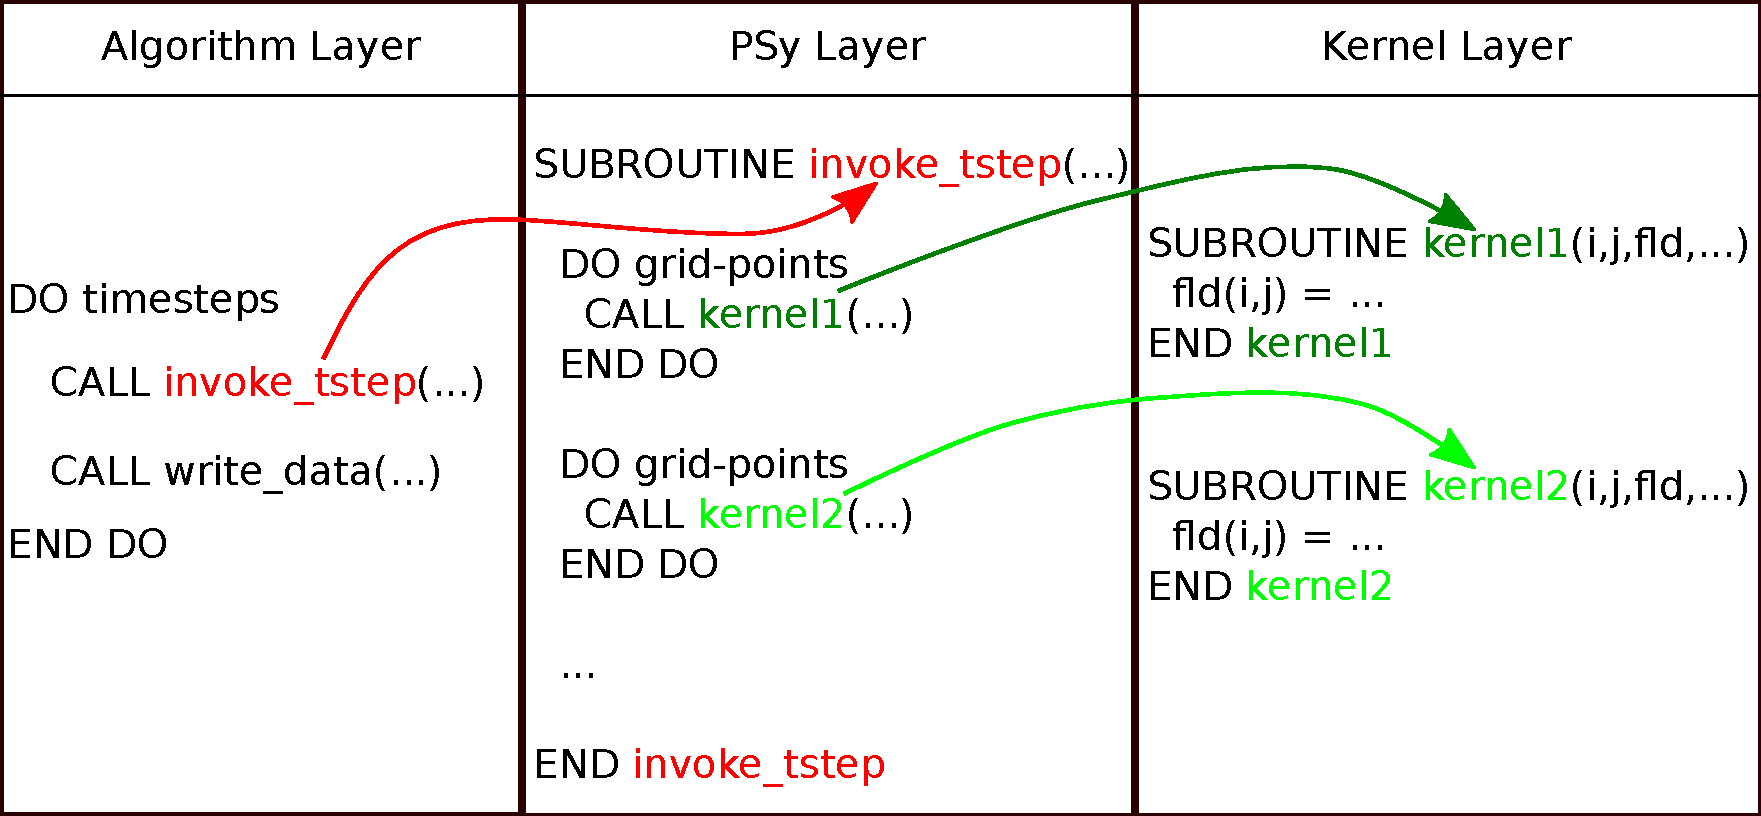
\includegraphics[width=100mm]{psykal_shallow}
\caption{A schematic of the vanilla \psykal version of the Shallow code.}
\label{FIG_psykal_shallow_structure}
\end{figure}

As with any full oceanographic model, boundary conditions must be
applied at the edges of the model domain. In the case of Shallow we
have periodic boundary conditions in both the $x$ and $y$ dimensions.
These are simply implemented by having additional (`halo')
rows/columns at the edges of the domain and ensuring the data in them
is up-to-date before it is read. These rows/columns are updated by
copying data from the corresponding row/column on the opposite side of
the domain. In the current work, the lines of code to do these copies
are manually inserted in the PSy-layer routine as required.

Excluding the application of boundary conditions, the code has three
main sections: computation of mass fluxes, vorticity and sea-surface
height; computation of the pressure and velocity components; and
finally, smoothing of the fields in time and copying of the field
values at the next time-step to be those at the current
time-step. Profiling of the original code showed that these three
sections each account for approximately one third of the run-time.

%%%%%%%%%%%%%%%%%%%%%%%%%%%%%%%%%%%%%%%%%%%%%%%%%%%%%%%%%%%%%%%%%%%%
\section{Methodology}

The primary aim of this work is to determine whether any performance
loss due to the \psykal separation of concerns can be negated by
optimising the PSy layer and if so, what the key transformations are
(for a given system). To evaluate this we perform tests on a range of
hardware and a range of compilers. The hardware and compilers are
listed in Table~\ref{TABLE_compilers}. Where a compiler is available
on a given piece of hardware, the version number used in this work is
specified.
%
The Intel Haswell-based system (Xeon E5-1620 v2) has a clock speed of
3.7~GHz and 10~MB of last-level cache. The Intel Ivy Bridge-based
system (Xeon E5-2697) has a clock speed of 2.7~GHz and a last-level
cache of 30~MB. The CPU in the IBM Power-8 system is built around 12
`chiplets'. Each chiplet has a single core with 64~KB of L1 cache,
512~KB of L2 cache and 8~MB of L3 cache. The L3 cache of each chiplet
is shared with all other chiplets so that there is a total of 96~MB of
last-level cache. The cores on the system we used had a clock speed of
3.3~GHz.

\begin{table}[!t]
% increase table row spacing, adjust to taste
\renewcommand{\arraystretch}{1.3}
\caption{The matrix of compilers and CPUs used in this work. The use
  of a compiler on a given CPU is indicated by the specification of
  the version of the compiler in the relevent element. No entry
  indicates that a compiler was not available/used on that CPU.}
\label{TABLE_compilers}
\centering
\begin{tabular}{|l|c|c|c|c|}
\hline
                 & \multicolumn{4}{c|}{Compiler}             \\
\hline
                 & Gnu   & Intel       & Cray    & IBM     \\
\hline
Intel Haswell    & 4.9.3 & 14.0.0      &         &          \\
Intel Ivy Bridge & 4.9.1 & 14.0.1.106  & 8.3.3   &          \\
IBM Power 8      &       &             &         & 15.1.2     \\
\hline
\end{tabular}
\end{table}

In Table~\ref{TABLE_compiler_flags} we give the optimisation flags
used with each compiler. These flags are particularly important for
the \psykal versions of the code. The performance of the original
version of the code is much less sensitive to the compiler
options. This is because it consists of a single source file
containing effectively a single routine (excluding those for I/O).
For all compilers apart from Cray it was important to use flags that
encourage in-lining. With the Cray compiler some benefit was obtained
by increasing the level of Inter-Procedural Analysis and using
'whole-program optimisation'. In order to get performant code from the
IBM compiler it was found essential to make the pre-fetching
considerably more aggressive than the default.
 
\begin{table}[!t]
% increase table row spacing, adjust to taste
\renewcommand{\arraystretch}{1.3}
\caption{The compiler flags used in this work.}
\label{TABLE_compiler_flags}
\centering
\begin{tabular}{l|l}
\hline
Compiler  &  Flags \\
\hline
Gnu       & -Ofast -mtune=native -finline-limit=50000    \\
Intel     & -O3 -fast -fno-inline-factor    \\
Cray      & -O3 -O ipa5 -h wp               \\
IBM       & \parbox{5cm}{-O5 -qinline=auto:level=10\\ -qprefetch=dscr=0x1D7} \\
\hline
\end{tabular}
\end{table}

Before applying any code transformations, we benchmark the original
version of the code. We also benchmark the vanilla, unoptimised
version after it has been re-structured following the \psykal
approach. These two versions of the code effectively provide upper and
lower bounds, respectively, on the performance we expect to achieve.

Beginning with the vanilla \psykal version, we then manually apply a
series of (cumulative) code transformations while obeying the \psykal
separation of concerns, {\it i.e.} optimisation is restricted to the
middle, {PS}y layer and leaves the kernel and algorithm layers
unchanged. The aim of these optimisations is to recover, as much as is
possible, the structure and thus performance of the original version
of the code. We began with two transformations that affect all of the
kernels. After this, we determined the transformations to perform by
comparing the timing profiles of the \psykal and original versions of
the code. We then tackled the sections resposible for the largest
slowdowns and iterated this process. While doing this we also made
heavy use of the optimisation reports produced by the compilers and
how these changed when moving from the original to the \psykal version
of the code.

The transformations we have performed are as follows:
\begin{enumerate}

\item Specify array bounds in the middle layer using module variables
  (rather than using assumed-size array arguments);

\item Move all kernel subroutines into the same module as as that
  containing the middle/PSy layer (`module inlining');

\item Loop fusion: all neighbouring loop nests were fully fused (where
  possible) with the exception of the first loop nest where it was
  found that fusing only the outer loop was more performant.

\item Manually in-line (`kernel inline') the three field-copy operations
  performed as part of the time-update section;

\item Loop fuse the three field-copy operations with the
  time-smoothing loop nest;

\item Manually in-line all kernel bodies into the middle-layer
  subroutine (kernel inlining);

\item Fully fuse the first loop nest (only the outer loop of this loop
  nest was fused in the first pass);

\item Make the array/loop bounds explicitly constant for the duration
  of the time-stepping loop (pass as arguments to the middle layer
  rather than using module variables);

\item Un-roll the outer loop of the time-smoothing loop nest using a
blocking factor of four (IBM supplied);

\item Fission the first loop nest back into three separate loop nests
  (IBM supplied).

\end{enumerate}

As indicated above, the last two of these transformations were
suggested by the IBM compiler team. The second of these effectively
undoes our 3rd transformation by fissioning the first loop nest back
into three separate loop nests.

We shall see that these transformations do not always result in improved
performance. Whether or not they do so depends both on the compiler
and the problem size. We also emphasise that the aim of these
optimisations is typically to recover, as far as is possible, the structure of
the original version of the code. It may well be that transforming the
code into some other structure would result in better performance on a
particular architecture. However, exploring this optimisation space is
beyond the scope of the present work.

We explore the extent to which performance depends upon the problem
size by using square domains of dimension 64, 128, 256, 512 and
1024. This range allows us to investigate what happens when cache is
exhausted as well as giving us some insight into the decisions that
different compilers make when optimising the code.

%%%%%%%%%%%%%%%%%%%%%%%%%%%%%%%%%%%%%%%%%%%%%%%%%%%%%%%%%%%%%%%%%%%%
\section{Results}

In this section we first discuss the performance of the original
version of the code with the various compiler/CPU combinations. We
then investigate the different code transformations that are required
to recover good performance from the \psykal version of Shallow. Finally,
we compare the most performant \psykal version  with the original
version of Shallow for each compiler/CPU combination.

\subsection{Performance of the Original Version of Shallow}

In Figure~\ref{FIG_orig_perf_summary} we plot the performance of the
original version of the Shallow code for the range of compilers and
hardware considered here. This summary demonstrates the effect of the
larger last-level cache of the Intel Ivy Bridge system compared to
that of the Haswell system; note the drop in performance
in going from a problem size of $256^{2}$ to a problem size of
$512^{2}$ for the first two bars. The performance of the Ivy
Bridge system with the Cray or Intel compiler (penultimate two bars)
only drops to this level when the domain size is increased to
$1024^{2}$. At this point, the working set no longer fits within cache
and performance is dominated by the bandwidth to main memory, making
it relatively insensitive to the choice of compiler.

\begin{figure}[!t]
\centering
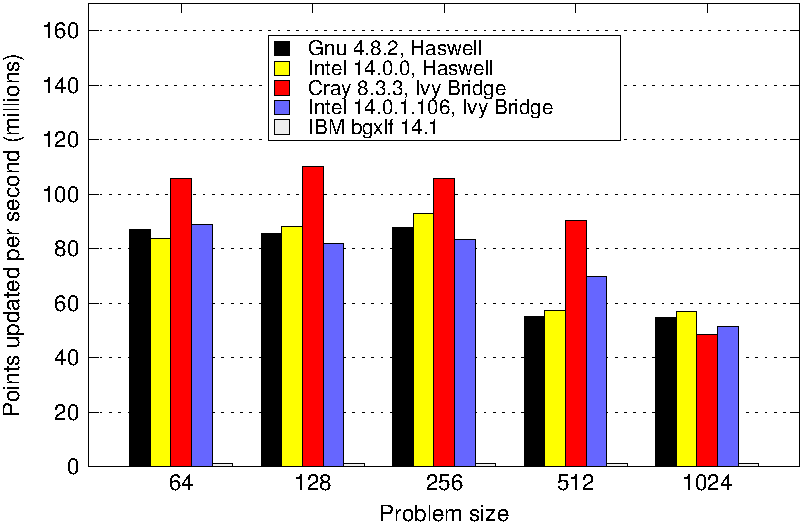
\includegraphics[width=120mm]{orig_summary}
\caption{Summary of the performance of the original Shallow code on
  the range of compilers and hardware under consideration.}
\label{FIG_orig_perf_summary}
\end{figure}

For this compiler-friendly form of the code, there is generally little
performance difference between the executables produced by the Gnu and
Intel compilers on both the Haswell and Ivy Bridge CPUs. However, the
executable produced by the Cray compiler generally performs
significantly better for all but the largest domain size. Analysis of
the optimisation reports produced by the Cray and Intel compilers did
not give any clues as to the cause of this difference and an in-depth
investigation is outside the scope of this paper.

\subsection{Optimisations of the \psykal Version to Recover Performance}

We now examine the performance of the \psykal version of Shallow and
the code transformations that are required to reach the levels obtained
by the original.  We do this for the $256^{2}$ problem size since this
fits within last-level cache on all of the CPUs we are using here.
The performance of the \psykal version after each transformation has
been applied to the code is plotted in
Figure~\ref{FIG_opt_stages_256}. Results for a given compiler/CPU are
given relative to the performance of the original version of Shallow
with the same compiler/CPU.

\begin{figure}[!t]
\centering
\includegraphics[width=123mm]{opt_stages_256}
\caption{The performance of the \psykal version of Shallow for the
  $256^{2}$ domain at each stage of optimisation. Results are given as
  a percentage of the performance of the original code for each
  compiler/CPU combination.}
\label{FIG_opt_stages_256}
\end{figure}

With the Gnu compiler (first and third clusters in
Figure~\ref{FIG_opt_stages_256}), the vanilla \psykal version of
Shallow only achieves ~5-6\% of the performance of the
original. Simply copying the code for each of the kernel subroutines
into the module from which they are called (module in-lining) has the
most dramatic effect on the performance of the compiled code; it now
achieves more than 80\% of the performance of the original. The
transformations required to get beyond this level then become
architecture dependent: on Haswell loop fusion achieves more than 90\%
while on Ivy Bridge it is fully-fusing the first loop nest. The
dramatic performance improvement obtained from the module-inlining
transformation demonstrates that the Gnu compiler is unable to
optimise over separate files.

With the Intel compiler, the key transformations to recover
performance are different (second and fourth clusters in
Figure~\ref{FIG_opt_stages_256}).  Even the vanilla \psykal version of
Shallow achieves some 80\% of the performance of the original
version. Only two code transformations were required to increase this
to $\sim$100\%. The first of these was the fusion of the computational
loops. However, we found that performance suffered (bar 5) when this
was extended to include the loop required for field copies at the end
of a time-step (Figure~\ref{FIG_time_smooth_code}). Further
investigation of this slow-down revealed that the compiler was unable
to SIMD vectorise the newly-fused loop after it had in-lined the body
of the kernel called from within it. Once this in-lining was done by
hand (bar 6), the compiler was able to vectorise the loop and the
performance of the original version of Shallow was recovered on the
Haswell system. On Ivy Bridge the first loop nest also had to be fully
fused (bar 7) to recover $\sim100\%$ of the performance.

\begin{figure}
\begin{verbatim}
! Time smoothing
DO J=1,N+1
  DO I=1,M+1
    CALL time_smooth_code(i,j,ufld,unew,uold)
!    uold(i,j) = ufld(i,j) + alpha* &
!     (unew(i,j) - 2.*ufld(i,j) + uold(i,j))
  END DO
END DO

! Copy new fields into current fields
DO J=1,N+1
  DO I=1,M+1
    Ufld(I,J) = UNEW(I,J)
  END DO
END DO
\end{verbatim}
\caption{Example of the coding structure that required manual
  in-lining of the kernel body (as indicated by commented-out lines)
  to retrieve the performance of the original version of Shallow with
  the Intel compiler.}
\label{FIG_time_smooth_code}
\end{figure}

The fifth cluster in Figure~\ref{FIG_opt_stages_256} shows the
evolution of the performance of the \psykal version of Shallow with
the Cray compiler. Again, this has significant differences from the
behaviour seen with the Gnu and Intel compilers. As with the Intel
compiler, the performance of the Vanilla \psykal version is fairly
good at 74\% of that of the original. In contrast to the other
compilers consisdered so far, the first significant transformation is
simply to specify the bounds of the arrays being used within the
middle layer using module variables (as opposed to specifying them as
assumed size). This tells the compiler that all of the arrays used in
the middle layer have the same extent and also that all of the
computational loops are over almost all elements of these arrays. This
simple change gives a \psykal version that achieves 88\% of the
performance of the original.

Subsequent transformations actually harm performance until the
field-copy operation of Figure~\ref{FIG_time_smooth_code} is fused
with the preceeding loop. The resulting \psykal version now achieves
94\% of the original performance. Two further steps are required to
match the latter. First, the first loop nest has to be fully fused
(both inner and outer loops fused) and second, the array/loop bounds
are passed as an argument to the middle layer. This is done in order
to indicate to the compiler that these bounds remain constant for the
duration of each trip of the time-stepping loop.

Moving to the IBM compiler on the Power 8 system (sixth cluster in
Figure~\ref{FIG_opt_stages_256}) we see that performance of the
vanilla \psykal version is only 5\% of the original and several
transformations are required to achieve comparable performance. As
with the Cray compiler, specifying array bounds explicitly improves
performance. Module-inlining also has a significant effect; doubling
the performance from 10 to 20\% of the original. However, fusing loop
nests actually harms performance, just as it did for the Cray
compiler. Kernel inlining takes performance to over 50\% and it is the
IBM-supplied transformations of loop unrolling and fissioning the
first loop ({\it i.e.} undoing some of transformations three and
seven) that finally recovers 96\% of the performance of the
original. We note that this final pair of transformations significantly
reduce the performance obtained with the Intel and Gnu compilers
although they do not much perturb that obtained by the Cray
compiler.

\subsection{Performance Comparison of the Original and \psykal Versions}

Finally, we compare the performance of the best \psykal version of
Shallow with that of the original. In
Figure~\ref{FIG_slowdown_summary} we plot the percentage {\em
  difference} between the performance of the original and the (best)
\psykal versions of Shallow for each compiler/CPU combination. The
most important feature of this plot is that the performance penalty
incurred by the \psykal version is less than four percent with only
one exception where it is 6.6\%.  In fact, for the Intel and Cray
compilers, the \psykal version of Shallow is never more than 2\%
slower than the original and in some cases is faster.  This
demonstrates that we can reliably recover the performance of the
original version of the code, despite the significant restructuring
required by the \psykal approach.

The exceptional case is that of the Gnu-compiled binary on the Haswell
CPU for a problem size of $256^2$.  This is strange since the
performance difference for the same case on the Ivy Bridge CPU is just
0.8\%. We investigated this further by compiling and running this case
with versions 4.8.3, 4.9.1 and 4.9.3 of the Gnu compiler on the
Haswell system. These gave slow-downs of 7.8\%, 7.3\% and 6.6\%,
respectively. From these results we conclude that the Gnu compiler's
support for/ability to exploit the newer Haswell architecture is still
maturing.

\begin{figure}[!t]
\centering
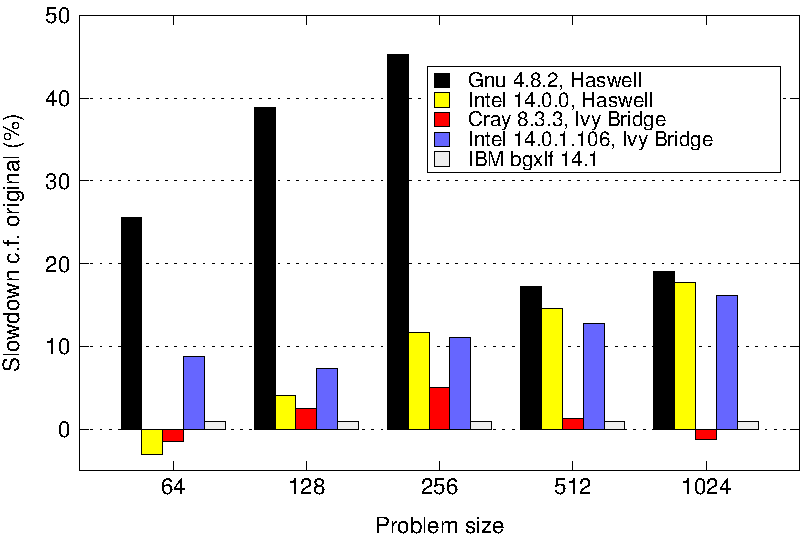
\includegraphics[width=120mm]{slowdown_summary}
\caption{Comparison of the performance of the best \psykal
version with that of the original version of the code. A negative value 
indicates that the \psykal version is faster than the original.}
\label{FIG_slowdown_summary}
\end{figure}

Turning to the cases where the \psykal version is significantly
{\em faster} than the original, we see from
Figure~\ref{FIG_slowdown_summary} that, with the exception of Power 8,
this only occurs for the smallest domain size. This is no doubt due in
part to the fact that the problem executes very quickly and therefore
a small reduction in run-time will show as a large precentage. Since
this problem is well contained in L2 cache, its performance will also
be more sensitive to small differences, {\it e.g.} in the way that CPU
registers are used. 

The performance of the Power 8 system with the $512^2$ domain size is
somewhat anomolous: the \psykal version of the code performs
significantly better than the original and in addition, this problem
size is also the only one where the Power 8 out-performs the Haswell
system (see Figure~\ref{FIG_orig_perf_summary}) for the original
version.  The results in Figure~\ref{FIG_orig_perf_summary} indicate
that the $512^2$ case marks a transition from the working set being in
cache (sizes $\leq 256^2$) to spilling out of cache (size $1024^2$). We
therefore suggest that cache is being used more efficiently on the
Power 8 system and this is further enhanced by the IBM-supplied
transformations in the \psykal version.

The main conclusion of all this analysis is that while we can employ a
separation of concerns and recover performance, doing so is not
straightforward. Determining how best to optimise even a simple code
such as Shallow is highly compiler- and CPU-dependent. Decisions that
are good on one platform may be bad for another and if these are
written into the source code then they will accumulate over time and
will almost certainly result in a code that does not perform optimally
on any system. For instance, loop fusion benefits performance for the
Gnu and Intel compilers and yet hurts performance with the Cray and
IBM compilers.

\section{Conclusions}

We have investigated the application of the \psykal separation of
concerns approach to the domain of finite-difference ocean
models. This approach enables the computational science (performance)
related aspects of a computer model to be kept separate from the
natural (oceanographic) science aspects.

As expected, applying this separation of concerns does reduce
performance significantly when compared with an existing, optimised
code. However, the application of code transformations to the
performance/PSy layer and the use of appropriate compiler flags can
recover any performance losses to within a few percent and in some
cases, despite limiting ourselves to transformations which replicate
the structure of the optimised code, result in slightly improved
performance.

In particular, the results on the IBM system demonstrate two key points.
%
First, even for a relatively simple
benchmark code, the code structure required to obtain good performance
between different architecture and/or compiler combinations may
differ. For hand optimised codes this implies the need to support
multiple code bases in order to achieve portable performance.
%
Second, the \psykal approach directly addresses the problem of
requiring different optimisations for different architectures and/or
compilers by limiting these differences to a separate performance
layer, thereby allowing the natural science code base to remain
unchanged.

In future work we will extend our performance portability analysis of
the \psykal approach to shared memory parallelisation optimisations on
different architectures using different parallelisation techniques (in
particular OpenMP on multi/many-core and OpenACC on GPU's).
%
We will then analyse the performance of a domain-specific compiler
that is currently under development. This compiler will generate
optimised PSy-layer code using a user-provided recipe of
transformations, thereby removing the need for optimisation experts to
manually write the PSy layer.

% use section* for acknowledgement
\section*{Acknowledgments}

This work made use of the ARCHER UK National Supercomputing Service
(\url{http://www.archer.ac.uk}). We acknowledge use of the Hartree
Centre IBM Power 8 system in this work. The STFC Hartree Centre is a
research collaboratory in association with IBM providing High
Performance Computing platforms funded by the UK's investment in
e-Infrastructure. The Centre aims to develop and demonstrate next
generation software, optimised to take advantage of the move towards
exa-scale computing. This work was funded by the NERC `GOcean' project,
grant number NE/L012111/1.

% http://www.ctan.org/tex-archive/biblio/bibtex/contrib/doc/
\bibliographystyle{unsrt}
% argument is your BibTeX string definitions and bibliography database(s)
\bibliography{shallow_perf}
%
\end{document}
